\clearpage
\hypertarget{conBran vis}{}
\subsection{Branching with statement nodes}
\visHeader

\begin{itemize}
  
\item[$\blacktriangleright$] Edit the \texttt{Box} class in your metamodel by invoking the \texttt{Operations} dialogue and create a new method called
\texttt{initalizeBox}. Recalling the sole condition of conditional branching, set its return type as \texttt{EBoolean}. Save the method, then open the \texttt{grow} SDM.

\item[$\blacktriangleright$] Add a new \texttt{StatementNode} named \texttt{initialize}. In the \texttt{Statement} tab, invoke a \texttt{MethodCallExpression}

\item[$\blacktriangleright$] Attach two \texttt{StopNode}s and appropriate edge guards to this new node. If the method call succeeds, the box was truly able
to increase its size, so return a literal \texttt{true}. If it failed however, \texttt{box} encountered an error (by having only one card) and returns
\texttt{false}. Overall, the new additions to \texttt{box.grow()} should resemble Fig.~\ref{fig:newGrowControl}.

\begin{figure}[htp]
\begin{center}
  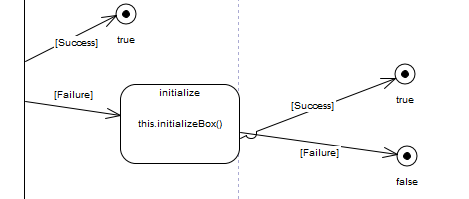
\includegraphics[width=0.8\textwidth]{ea_growControlAddition}
  \caption{The extended \texttt{grow} SDM}
  \label{fig:newGrowControl}
\end{center}
\end{figure}

\item[$\blacktriangleright$] Now that have edited our control flow, save, validate, and build your metamodel in Eclipse. Open \texttt{BoxImpl.java},
and navigate to \texttt{grow}, which starts at (approximately) line 207. Scan the comments until you find \texttt{//statement node `initialize'}.

\begin{figure}[htp]
\begin{center}
  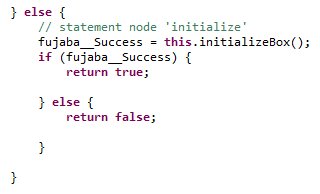
\includegraphics[width=0.5\textwidth]{eclipse_boxImplStatementNode}
  \caption{Our statement node declaration}
  \label{fig:initBoxImpl}
\end{center}
\end{figure}

\item[$\blacktriangleright$] This is all we need (and can have) for a statement node. It simply guarantees a command execution. Hold \texttt{ctrl} while
clicking on the method to automatically jump to its declaration (Fig.~\ref{fig:initBoxDecl}).

\begin{figure}[htp]
\begin{center}
  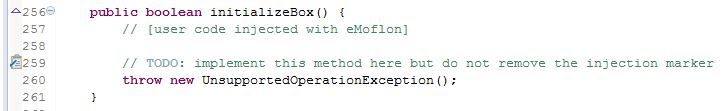
\includegraphics[width=\textwidth]{eclipse_initializeBoxDeclaration}
  \caption{The \texttt{initializeBox} declaration}
  \label{fig:initBoxDecl}
\end{center}
\end{figure}

\item[$\blacktriangleright$] You now have a choice -- you can either implement the method by hand by completing this declaration, or you can return to
your metamodel and create it there. Writing your own method makes sense if its a simple function, but given the strict pattern requirements (we must check
to see if there is a single partition) we'll need to create another NAC, which can become very difficult, \emph{very} quickly.

 \item[$\blacktriangleright$] Switch back to your open \texttt{Box.grow} SDM in EA. You'll notice that if you double-click on \texttt{initialize}, the
 \texttt{Extract Story Pattern} option is invalid. This makes sense -- you don't define actions in a statement node. Instead, return to the main diagram and
 create a new SDM for \texttt{initializeBox}.
 
 \item[$\blacktriangleright$] Create a bounded \texttt{Box}, connected to a \texttt{onePartition} NAC, and two creational partitions, \texttt{firstPartition}
 and \texttt{lastPartition}. Also connect two true/false \texttt{StopNode}s. Your workspace should now resemble Fig.~\ref{fig:buildPartitions}.
 
\item[$\blacktriangleright$] Save, validate, and build your metamodel. Review \texttt{BoxImpl.java} in the Eclipse workspace once again and see the changes in
\texttt{initializeBox}.
 
\newpage
 
 \vspace*{3cm}
 
 \begin{figure}[htp]
\begin{center}
  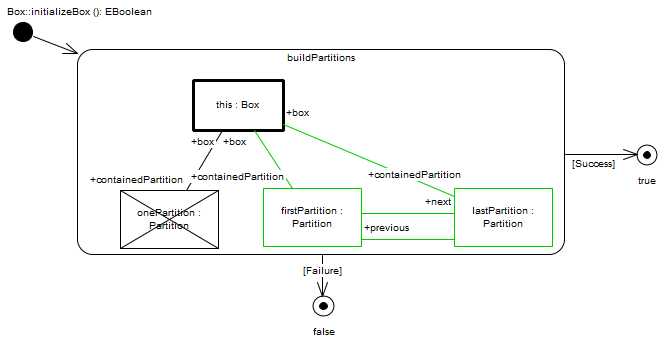
\includegraphics[width=\textwidth]{eclipse_buildPartitions}
  \caption{NAC to check for a single partition}
  \label{fig:buildPartitions}
\end{center}
\end{figure}

\jumpSingle{sec:extendedGui}

\end{itemize}
